\subsection{2021年4月13日}
\paragraph{\href{https://www.51voa.com/VOA_Special_English/iran-blames-israel-for-nuclear-plant-outage-86655.html}{原文}}

\begin{figure}[H]
\centering
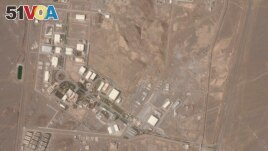
\includegraphics[scale=0.7]{005_voa_20210413.jpg}
\caption{This satellite photo from Planet Labs Inc. shows Iran's Natanz nuclear facility on Wednesday, April 7, 2021. (Planet Labs Inc. via AP)}
\end{figure}
By Bryan Lynn
12 April 2021
Iran has accused Israel of carrying out an attack on a nuclear center that damaged equipment and caused a power outage.
Iranian officials called Sunday's incident at the Natanz nuclear center an act of "nuclear terrorism." They said centrifuges were damaged at the plant. A centrifuge is a device used to increase the purity of uranium for nuclear purposes.
Media organizations reported the Israeli government was behind the action, which was described as a cyberattack. However, Israel did not claim responsibility for an attack or comment directly on the incident.
Speaking to reporters Monday, Israeli Prime Minister Benjamin Netanyahu said Israel would continue efforts aimed at preventing Iran from gaining a nuclear weapon. He said such a device would give Iran the ability "to carry out its genocidal goal of eliminating Israel." He added that Israel "will continue to defend itself against Iran's aggression and terrorism."
A former chief of Iran's paramilitary Revolutionary Guard, General Mohsen Rezaei, said in a message on Twitter that the attack had started a fire.
Iran's Foreign Ministry spokesman Saeed Khatibzadeh said the country's answer to the action should be "to take revenge against Israel." He did not comment further, but added that Israel "will receive its answer through its own path."
Khatibzadeh confirmed that centrifuges at the plant had been damaged. The incident took place one day after Iran announced it had launched new, advanced centrifuge machines at Natanz. Khatibzadeh said only the older centrifuges were damaged.
Iran's improvements in centrifuge technology are designed to permit the country to process uranium faster.
Since January, Iran has begun enriching uranium to as high as 20 percent purity, a technical step away from weapons-grade levels.
The incident came after negotiations began last week in Vienna aiming to bring the United States back into a 2015 nuclear deal with Iran. The deal -- which the U.S. left in 2018 under President Donald Trump -- restricts Iran's nuclear program in exchange for easing U.S. and international sanctions.
The U.S. reestablished economic sanctions after withdrawing from the agreement. Iran answered by violating some of the terms of the deal.
In Vienna, officials from the U.S. and Iran were holding indirect talks. Also taking part were representatives from countries still in the nuclear deal -- Britain, China, France, Germany and Russia.
U.S. Defense Secretary Lloyd Austin arrived Monday in Israel for talks with Netanyahu and other officials. When asked by reporters whether the nuclear discussions might be affected by the incident at the plant Lloyd said, "Those efforts will continue."
In a statement, the White House said it knew about the Natanz attack and that "the U.S. was not involved in any manner."
I'm Bryan Lynn.

\begin{messagebox}
Words in This Story
cyberattack – n. an attempt by attackers to damage or destroy a computer network or system
eliminate – v. remove or get rid of something
revenge – n. the act of doing something to hurt someone because that person did something that hurt you
advanced – adj. having developed or progressed to a late stage
sanction – n. a restriction, usually limiting trade, that are meant to cause a country to obey international law
manner –n. way or method that something is done
\end{messagebox}

Iran has accused Israel of carrying out an attack on a nuclear center that damaged equipment and caused a power outage.
伊朗指责以色列袭击一处核中心,破坏了设备,并造成了停电。
Iranian officials called Sunday's incident at the Natanz nuclear center an act of "nuclear terrorism." They said centrifuges were damaged at the plant. A centrifuge is a device used to increase the purity of uranium for nuclear purposes.
伊朗官员称纳坦兹核中心周日发生的事件是“核恐怖主义”行为。他们表示该工厂有离心机受到了破坏。离心机是一种提高铀纯度用于核用途的设备。

Media organizations reported the Israeli government was behind the action, which was described as a cyberattack. However, Israel did not claim responsibility for an attack or comment directly on the incident.
媒体机构报道称,以色列政府是这场被称为网络攻击的行动的幕后黑手。然而,以色列并未宣称对这起袭击事件负责,也没有直接对该事件发表评论。

Speaking to reporters Monday, Israeli Prime Minister Benjamin Netanyahu said Israel would continue efforts aimed at preventing Iran from gaining a nuclear weapon. He said such a device would give Iran the ability "to carry out its genocidal goal of eliminating Israel." He added that Israel "will continue to defend itself against Iran's aggression and terrorism."
以色列总理内塔尼亚胡周一对记者表示,以色列将继续努力防止伊朗获得核武器。他说,这种武器将使伊朗有能力“实施其消灭以色列的种族主义目标。”他还表示,以色列“将继续抵抗伊朗的侵略和恐怖主义。”

A former chief of Iran's paramilitary Revolutionary Guard, General Mohsen Rezaei, said in a message on Twitter that the attack had started a fire.
伊朗革命卫队前负责人莫森·雷扎伊在推特上发文表示,这次袭击引发了大火。

Iran's Foreign Ministry spokesman Saeed Khatibzadeh said the country's answer to the action should be "to take revenge against Israel." He did not comment further, but added that Israel "will receive its answer through its own path."
伊朗外交部发言人赛义德·哈蒂布扎德表示,作为回应,伊朗将会对以色列展开报复。他没有进一步评论。但是他还表示,以色列将通过自己的途径得到答案。

Khatibzadeh confirmed that centrifuges at the plant had been damaged. The incident took place one day after Iran announced it had launched new, advanced centrifuge machines at Natanz. Khatibzadeh said only the older centrifuges were damaged.
哈蒂布扎德确认该工厂的离心机已被损坏。事件发生前一天,伊朗刚宣布在纳坦兹核中心启动更先进的新型离心机。哈蒂布扎德表示,只有旧型号离心机受到了破坏。

Iran's improvements in centrifuge technology are designed to permit the country to process uranium faster.
伊朗对离心机技术的改进旨在使该国更快地加工铀。

Since January, Iran has begun enriching uranium to as high as 20 percent purity, a technical step away from weapons-grade levels.
自1月以来,伊朗已经开始将铀浓缩至高达20%的纯度,这是接近武器级水平的一项技术步骤。

The incident came after negotiations began last week in Vienna aiming to bring the United States back into a 2015 nuclear deal with Iran. The deal -- which the U.S. left in 2018 under President Donald Trump -- restricts Iran's nuclear program in exchange for easing U.S. and international sanctions.
事件发生前,上周在维也纳开展了旨在使美国重回与伊朗达成的2015年核协议的谈判。这项协议以限制伊朗的核计划换取美国和国际放松制裁,川普总统于2018年带领美国退出了该协议。

The U.S. reestablished economic sanctions after withdrawing from the agreement. Iran answered by violating some of the terms of the deal.
美国在退出协议后重启了经济制裁。伊朗通过违反该协议的某些条款做出了回应。

In Vienna, officials from the U.S. and Iran were holding indirect talks. Also taking part were representatives from countries still in the nuclear deal -- Britain, China, France, Germany and Russia.
在维也纳,来自美国和伊朗的官员进行了间接谈判。仍然留在该协议中的国家的代表也参加了这次会议,这些国家包括英国、中国、法国、德国和俄罗斯。

U.S. Defense Secretary Lloyd Austin arrived Monday in Israel for talks with Netanyahu and other officials. When asked by reporters whether the nuclear discussions might be affected by the incident at the plant Lloyd said, "Those efforts will continue."
美国国防部长劳埃德·奥斯丁周一抵达以色列,与内塔尼亚胡等官员举行了会谈。当记者问到核谈判是否会受到此次事件的影响时,劳埃德表示:“谈判还将继续下去。”

In a statement, the White House said it knew about the Natanz attack and that "the U.S. was not involved in any manner."
白宫在一份声明中表示,它知晓纳坦兹核中心发生的袭击事件,美国没有以任何方式介入。

I'm Bryan Lynn.
我是布莱恩·林恩。
